\documentclass[journal,12pt,twocolumn]{IEEEtran}
%
\usepackage{setspace}
\usepackage{gensymb}
\usepackage{xcolor}
\usepackage{caption}
%\usepackage{subcaption}
%\doublespacing
\singlespacing

%\usepackage{graphicx}
%\usepackage{amssymb}
%\usepackage{relsize}
\usepackage[cmex10]{amsmath}
\usepackage{mathtools}
%\usepackage{amsthm}
%\interdisplaylinepenalty=2500
%\savesymbol{iint}
%\usepackage{txfonts}
%\restoresymbol{TXF}{iint}
%\usepackage{wasysym}
\usepackage{hyperref}
\usepackage{amsthm}
\usepackage{mathrsfs}
\usepackage{txfonts}
\usepackage{stfloats}
\usepackage{cite}
\usepackage{cases}
\usepackage{subfig}
%\usepackage{xtab}
\usepackage{longtable}
\usepackage{multirow}
%\usepackage{algorithm}
%\usepackage{algpseudocode}
%\usepackage{enumerate}
\usepackage{enumitem}
\usepackage{mathtools}
%\usepackage{iithtlc}
%\usepackage[framemethod=tikz]{mdframed}
\usepackage{listings}


%\usepackage{stmaryrd}


%\usepackage{wasysym}
%\newcounter{MYtempeqncnt}
\DeclareMathOperator*{\Res}{Res}
%\renewcommand{\baselinestretch}{2}
\renewcommand\thesection{\arabic{section}}
\renewcommand\thesubsection{\thesection.\arabic{subsection}}
\renewcommand\thesubsubsection{\thesubsection.\arabic{subsubsection}}

\renewcommand\thesectiondis{\arabic{section}}
\renewcommand\thesubsectiondis{\thesectiondis.\arabic{subsection}}
\renewcommand\thesubsubsectiondis{\thesubsectiondis.\arabic{subsubsection}}

%\renewcommand{\labelenumi}{\textbf{\theenumi}}
%\renewcommand{\theenumi}{P.\arabic{enumi}}

% correct bad hyphenation here
\hyphenation{op-tical net-works semi-conduc-tor}

\lstset{
language=Python,
frame=single, 
breaklines=true,
columns=fullflexible
}
\usepackage{enumitem}
\usepackage{amsmath}
\usepackage{amssymb}
\usepackage{gensymb}
\usepackage{graphicx}
\usepackage{txfonts}         
\usepackage{listings}
\usepackage{lstautogobble}
\usepackage{mathtools}
\usepackage{bm}
\usepackage{hyperref}
\usepackage{polynom}
\usepackage{capt-of}
\usepackage{siunitx}
\newcommand{\solution}{\noindent \textbf{Solution: }}
\providecommand{\pr}[1]{\ensuremath{\Pr\left(#1\right)}}
\providecommand{\brak}[1]{\ensuremath{\left(#1\right)}}
\providecommand{\cbrak}[1]{\ensuremath{\left\{#1\right\}}}
\providecommand{\sbrak}[1]{\ensuremath{\left[#1\right]}}
\providecommand{\mean}[1]{E\left[ #1 \right]}
\providecommand{\var}[1]{\mathrm{Var}\left[ #1 \right]}
\providecommand{\der}[1]{\mathrm{d} #1}
\providecommand{\gauss}[2]{\mathcal{N}\ensuremath{\left(#1,#2\right)}}
\providecommand{\mbf}{\mathbf}
\providecommand{\abs}[1]{\left\vert#1\right\vert}
\providecommand{\norm}[1]{\left\lVert#1\right\rVert}
\providecommand{\z}[1]{{\mathcal{Z}}\{#1\}}
\providecommand{\ztrans}{\overset{\mathcal{Z}}{ \rightleftharpoons}}

\providecommand{\parder}[2]{\frac{\partial}{\partial #2} \brak{#1}}

\let\StandardTheFigure\thefigure
\let\vec\mathbf

\numberwithin{equation}{section}
\renewcommand{\thefigure}{\theenumi}
\renewcommand\thesection{\arabic{section}}

\newcommand{\myvec}[1]{\ensuremath{\begin{pmatrix}#1\end{pmatrix}}}
\newcommand{\mydet}[1]{\ensuremath{\begin{vmatrix}#1\end{vmatrix}}}
\newcommand{\define}{\stackrel{\triangle}{=}}

\DeclareMathOperator*{\argmin}{arg\,min}
\DeclareMathOperator*{\argmax}{arg\,max}



\begin{document}
%

\theoremstyle{definition}
\newtheorem{theorem}{Theorem}[section]
\newtheorem{problem}{Problem}
\newtheorem{proposition}{Proposition}[section]
\newtheorem{lemma}{Lemma}[section]
\newtheorem{corollary}[theorem]{Corollary}
\newtheorem{example}{Example}[section]
\newtheorem{definition}{Definition}[section]
%\newtheorem{algorithm}{Algorithm}[section]
%\newtheorem{cor}{Corollary}
\newcommand{\BEQA}{\begin{eqnarray}}
\newcommand{\EEQA}{\end{eqnarray}}

\bibliographystyle{IEEEtran}
%\bibliographystyle{ieeetr}

\providecommand{\nCr}[2]{\,^{#1}C_{#2}} % nCr
\providecommand{\nPr}[2]{\,^{#1}P_{#2}} % nPr
\providecommand{\mbf}{\mathbf}
\providecommand{\pr}[1]{\ensuremath{\Pr\left(#1\right)}}
\providecommand{\qfunc}[1]{\ensuremath{Q\left(#1\right)}}
\providecommand{\sbrak}[1]{\ensuremath{{}\left[#1\right]}}
\providecommand{\lsbrak}[1]{\ensuremath{{}\left[#1\right.}}
\providecommand{\rsbrak}[1]{\ensuremath{{}\left.#1\right]}}
\providecommand{\brak}[1]{\ensuremath{\left(#1\right)}}
\providecommand{\lbrak}[1]{\ensuremath{\left(#1\right.}}
\providecommand{\rbrak}[1]{\ensuremath{\left.#1\right)}}
\providecommand{\cbrak}[1]{\ensuremath{\left\{#1\right\}}}
\providecommand{\lcbrak}[1]{\ensuremath{\left\{#1\right.}}
\providecommand{\rcbrak}[1]{\ensuremath{\left.#1\right\}}}
\theoremstyle{remark}
\newtheorem{rem}{Remark}
\newcommand{\sgn}{\mathop{\mathrm{sgn}}}
\providecommand{\abs}[1]{\left\vert#1\right\vert}
\providecommand{\res}[1]{\Res\displaylimits_{#1}} 
\providecommand{\norm}[1]{\lVert#1\rVert}
\providecommand{\mtx}[1]{\mathbf{#1}}
\providecommand{\mean}[1]{E\left[ #1 \right]}
\providecommand{\fourier}{\overset{\mathcal{F}}{ \rightleftharpoons}}
\providecommand{\ztrans}{\overset{\mathcal{Z}}{ \rightleftharpoons}}


%\providecommand{\hilbert}{\overset{\mathcal{H}}{ \rightleftharpoons}}
\providecommand{\system}{\overset{\mathcal{H}}{ \longleftrightarrow}}
	%\newcommand{\solution}[2]{\textbf{Solution:}{#1}}
\providecommand{\dec}[2]{\ensuremath{\overset{#1}{\underset{#2}{\gtrless}}}}
\numberwithin{equation}{section}
%\numberwithin{equation}{subsection}
%\numberwithin{problem}{subsection}
%\numberwithin{definition}{subsection}
\makeatletter
\@addtoreset{figure}{problem}
\makeatother

\let\StandardTheFigure\thefigure
%\renewcommand{\thefigure}{\theproblem.\arabic{figure}}
\renewcommand{\thefigure}{\theproblem}


%\numberwithin{figure}{subsection}

\def\putbox#1#2#3{\makebox[0in][l]{\makebox[#1][l]{}\raisebox{\baselineskip}[0in][0in]{\raisebox{#2}[0in][0in]{#3}}}}
     \def\rightbox#1{\makebox[0in][r]{#1}}
     \def\centbox#1{\makebox[0in]{#1}}
     \def\topbox#1{\raisebox{-\baselineskip}[0in][0in]{#1}}
     \def\midbox#1{\raisebox{-0.5\baselineskip}[0in][0in]{#1}}

\vspace{3cm}

\title{ 
%\logo{
Digital Signal Processing
%}
%	\logo{Octave for Math Computing }
}
%\title{
%	\logo{Matrix Analysis through Octave}{\begin{center}\includegraphics[scale=.24]{tlc}\end{center}}{}{HAMDSP}
%}


% paper title
% can use linebreaks \\ within to get better formatting as desired
%\title{Matrix Analysis through Octave}
%
%
% author names and IEEE memberships
% note positions of commas and nonbreaking spaces ( ~ ) LaTeX will not break
% a structure at a ~ so this keeps an author's name from being broken across
% two lines.
% use \thanks{} to gain access to the first footnote area
% a separate \thanks must be used for each paragraph as LaTeX2e's \thanks
% was not built to handle multiple paragraphs
%

\author{ Bandaru Naresh Kumar$^{*}$ %<-this  stops a space
\thanks{*The author is with the Department
of Electrical Engineering, Indian Institute of Technology, Hyderabad
502285 India e-mail:  gadepall@iith.ac.in.  All content in the manuscript is 
released under GNU GPL.  Free to use for anything. }% <-this % stops a space
%\thanks{J. Doe and J. Doe are with Anonymous University.}% <-this % stops a space
%\thanks{Manuscript received April 19, 2005; revised January 11, 2007.}}
}
% note the % following the last \IEEEmembership and also \thanks - 
% these prevent an unwanted space from occurring between the last author name
% and the end of the author line. i.e., if you had this:
% 
% \author{....lastname \thanks{...} \thanks{...} }
%                     ^------------^------------^----Do not want these spaces!
%
% a space would be appended to the last name and could cause every name on that
% line to be shifted left slightly. This is one of those "LaTeX things". For
% instance, "\textbf{A} \textbf{B}" will typeset as "A B" not "AB". To get
% "AB" then you have to do: "\textbf{A}\textbf{B}"
% \thanks is no different in this regard, so shield the last } of each \thanks
% that ends a line with a % and do not let a space in before the next \thanks.
% Spaces after \IEEEmembership other than the last one are OK (and needed) as
% you are supposed to have spaces between the names. For what it is worth,
% this is a minor point as most people would not even notice if the said evil
% space somehow managed to creep in.



% The paper headers
%\markboth{Journal of \LaTeX\ Class Files,~Vol.~6, No.~1, January~2007}%
%{Shell \MakeLowercase{\textit{et al.}}: Bare Demo of IEEEtran.cls for Journals}
% The only time the second header will appear is for the odd numbered pages
% after the title page when using the twoside option.
% 
% *** Note that you probably will NOT want to include the author's ***
% *** name in the headers of peer review papers.                   ***
% You can use \ifCLASSOPTIONpeerreview for conditional compilation here if
% you desire.




% If you want to put a publisher's ID mark on the page you can do it like
% this:
%\IEEEpubid{0000--0000/00\$00.00~\copyright~2007 IEEE}
% Remember, if you use this you must call \IEEEpubidadjcol in the second
% column for its text to clear the IEEEpubid mark.



% make the title area
\maketitle

%\newpage

\tableofcontents

%\renewcommand{\thefigure}{\thesection.\theenumi}
%\renewcommand{\thetable}{\thesection.\theenumi}

\renewcommand{\thefigure}{\theenumi}
\renewcommand{\thetable}{\theenumi}

%\renewcommand{\theequation}{\thesection}


\bigskip

\begin{abstract}
This manual provides a simple introduction to digital signal processing.
\end{abstract}
\section{Software Installation}
Run the following commands
\begin{lstlisting}
sudo apt-get update
sudo apt-get install libffi-dev libsndfile1 python3-scipy  python3-numpy python3-matplotlib 
sudo pip install cffi pysoundfile 
\end{lstlisting}
\section{Digital Filter}
\begin{enumerate}[label=\thesection.\arabic*
,ref=\thesection.\theenumi]
\item
\label{prob:input}
Download the sound file from  
\begin{lstlisting}
wget https://raw.githubusercontent.com/gadepall/ 
EE1310/master/filter/codes/Sound_Noise.wav
\end{lstlisting}
%\href{http://tlc.iith.ac.in/img/sound/Sound_Noise.wav}{\url{http://tlc.iith.ac.in/img/sound/Sound_Noise.wav}}  
%in the link given below.
%\linebreak
\item
\label{prob:spectrogram}
You will find a spectrogram at \href{https://academo.org/demos/spectrum-analyzer}{\url{https://academo.org/demos/spectrum-analyzer}}. 
%\end{problem}
%%
%
%%\onecolumn
%%\input{./figs/fir}
%\begin{problem}
Upload the sound file that you downloaded in Problem \ref{prob:input} in the spectrogram  and play.  Observe the spectrogram. What do you find?
\\
%
\solution There are a lot of yellow lines between 440 Hz to 5.1 KHz.  These represent the synthesizer key tones. Also, the key strokes are audible along with background noise.\\\\
% By observing spectrogram, it clearly shows that tonal frequency is under 4kHz. And above 4kHz only noise is present.
\item
\label{prob:output}
Write the python code for removal of out of band noise and execute the code.
\\
\solution
\lstinputlisting{/home/naresh/signal processing/codes/2-3.py}
%\begin{figure}[h]
%\centering
%\includegraphics[width=\columnwidth]{enc_block_diag.png}
%\caption{}
%\label{fig:convolution encoder}
%\end{figure}
%\input{block_enc}
\item
The output of the python script in Problem \ref{prob:output} is the audio file Sound\_With\_ReducedNoise.wav. Play the file in the spectrogram in Problem \ref{prob:spectrogram}. What do you observe?
\\
\solution The key strokes as well as background noise is subdued in the audio.  Also,  the signal is blank for frequencies above 5.1 kHz.
\end{enumerate}
\section{Difference Equation}
\begin{enumerate}[label=\thesection.\arabic*,ref=\thesection.\theenumi]
\item Let
\begin{equation}
x(n) = \cbrak{\underset{\uparrow}{1},2,3,4,2,1}
\end{equation}
Sketch $x(n)$.
\item Let
\begin{multline}
\label{eq:iir_filter}
y(n) + \frac{1}{2}y(n-1) = x(n) + x(n-2), 
\\
 y(n) = 0, n < 0
\end{multline}
Sketch $y(n)$.
\\
\solution The following code yields Fig. \ref{fig:xnyn}.
\begin{lstlisting}
wget https://github.com/NareshBandaru13/EE3900-A1/blob/main/codes/3-2.py
\end{lstlisting}
\begin{figure}[!ht]
\begin{center}
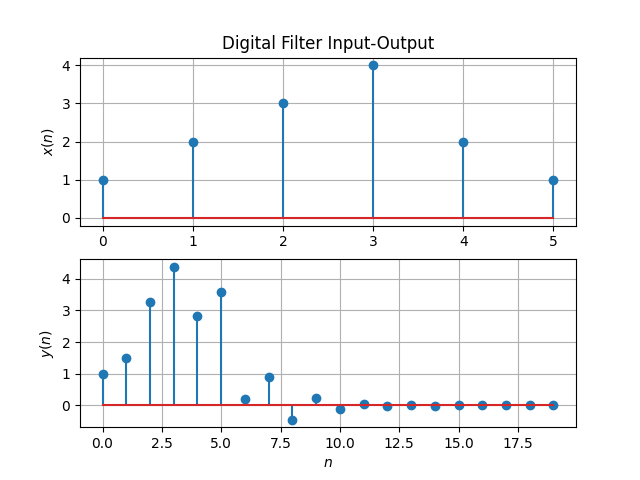
\includegraphics[width=\columnwidth]{/home/naresh/signal processing/figures/xnyn.png}
\end{center}
\captionof{figure}{}
\label{fig:xnyn}	
\end{figure}
\item Repeat the above exercise using a c code.
\solution The following code yields x data and y data
\begin{lstlisting}
wget https://github.com/NareshBandaru13/EE3900-A1/blob/main/codes/3-3.c
\end{lstlisting}
\end{enumerate}
\section{$Z$-transform}
\begin{enumerate}[label=\thesection.\arabic*]
\item The $Z$-transform of $x(n)$ is defined as
%
\begin{equation}
\label{eq:z_trans}
X(z)={\mathcal {Z}}\{x(n)\}=\sum _{n=-\infty }^{\infty }x(n)z^{-n}
\end{equation}
%
Show that
\begin{equation}
\label{eq:shift1}
{\mathcal {Z}}\{x(n-1)\} = z^{-1}X(z)
\end{equation}
and find
\begin{equation}
	{\mathcal {Z}}\{x(n-k)\} 
\end{equation}
\solution From \eqref{eq:z_trans},
\begin{align}
{\mathcal {Z}}\{x(n-k)\} &=\sum _{n=-\infty }^{\infty }x(n-1)z^{-n}
\\
&=\sum _{n=-\infty }^{\infty }x(n)z^{-n-1} = z^{-1}\sum _{n=-\infty }^{\infty }x(n)z^{-n}
\end{align}
resulting in \eqref{eq:shift1}. Similarly, it can be shown that
%
\begin{equation}
\label{eq:z_trans_shift}
	{\mathcal {Z}}\{x(n-k)\} = z^{-k}X(z)
\end{equation}
\item Obtain X(z) for x(n) defined in problem 3.1\\
\solution $$X(z)={\mathcal {z}}\{x(n)\}=\sum_{n=-\infty}^{\infty}x(n)z^{-n}$$
\begin{align*}
X(z) &= ...0+x(0)z^{0}+x(1)z^{-1}+x(2)z^{-2}+x(3)z^{-3}+x(4)z^{-4}+x(5)z^{-5}+0...\\
     &= 1+2z^-1+3z^-2+4z^-3+2z^-4+1z^-5\\
\end{align*}

\item Find
%
\begin{equation}
H(z) = \frac{Y(z)}{X(z)}
\end{equation}
%
from  \eqref{eq:iir_filter} assuming that the $Z$-transform is a linear operation.
\\
\solution  Applying \eqref{eq:z_trans_shift} in \eqref{eq:iir_filter},
\begin{align}
Y(z) + \frac{1}{2}z^{-1}Y(z) &= X(z)+z^{-2}X(z)
\\
\implies \frac{Y(z)}{X(z)} &= \frac{1 + z^{-2}}{1 + \frac{1}{2}z^{-1}}
\label{eq:freq_resp}
\end{align}
%
\item Find the Z transform of 
\begin{equation}
\delta(n)
=
\begin{cases}
1 & n = 0
\\
0 & \text{otherwise}
\end{cases}
\end{equation}
and show that the $Z$-transform of
\begin{equation}
\label{eq:unit_step}
u(n)
=
\begin{cases}
1 & n \ge 0
\\
0 & \text{otherwise}
\end{cases}
\end{equation}
is
\begin{equation}
U(z) = \frac{1}{1-z^{-1}}, \quad \abs{z} > 1
\end{equation}
\solution It is easy to show that
\begin{equation}
\delta(n) \ztrans 1
\end{equation}
and from \eqref{eq:unit_step},
\begin{align}
U(z) &= \sum _{n= 0}^{\infty}z^{-n}
\\
&=\frac{1}{1-z^{-1}}, \quad \abs{z} > 1
\end{align}
using the fomula for the sum of an infinite geometric progression.
%
\item Show that 
\begin{equation}
\label{eq:anun}
a^nu(n) \ztrans \frac{1}{1-az^{-1}} \quad \abs{z} > \abs{a}
\end{equation}
\solution$X(z) = \sum_{n=-\infty}^{\infty}x(n)z^{-n}$
\begin{align*}
X(z) &= \sum_{n=-\infty}^{-1}0 + \sum_{n=0}^{\infty}a^{n}(1)z^{-n} \\
     &= \sum_{n=0}^{\infty} (az^{-1})^{n} \\
     &= \frac{1}{1-az^-1}
\end{align*}
Also the series is convergent for $|z| > |a|$\\\\
%
\item 
Let
\begin{equation}
H\brak{e^{\j \omega}} = H\brak{z = e^{\j \omega}}.
\end{equation}
Plot $\abs{H\brak{e^{\j \omega}}}$.  Comment.  $H(e^{\j \omega})$ is
known as the {\em Discret Time Fourier Transform} (DTFT) of $x(n)$.\\
\solution The following code plots Fig. \ref{fig:dtft}.
\begin{lstlisting}
wget https://github.com/NareshBandaru13/EE3900-A1/blob/main/codes/4-6.py
\end{lstlisting}
run the command
\begin{lstlisting}
python3 4-6.py
\end{lstlisting}
\begin{align}
		H\brak{e^{\j \omega}} &= \frac{1 + e^{-2\j\omega}}{1 + \frac12 e^{-\j\omega}} \\
		\implies \abs{H\brak{e^{\j \omega}}} &= \frac{\abs{1 + \cos2\omega - \j\sin2\omega}}{\abs{1 + \frac12 \cos\omega - \frac12 \sin\omega}} \\
		&= \sqrt{\frac{(1 + \cos2\omega)^2 + (\sin2\omega)^2}{(1 + \frac12 \cos\omega)^2 + (\frac12 \sin\omega)^2}} \\
		&= \sqrt{\frac{2 + 2\cos2\omega}{\frac54 + \cos\omega}} \\
		&= \sqrt{\frac{2(2\cos^2\omega)4}{5 + 4\cos\omega} } \\
		&= \frac{4\abs{\cos\omega}}{\sqrt{5 + 4\cos\omega}}
	\end{align} 
\begin{figure}[!ht]
\centering
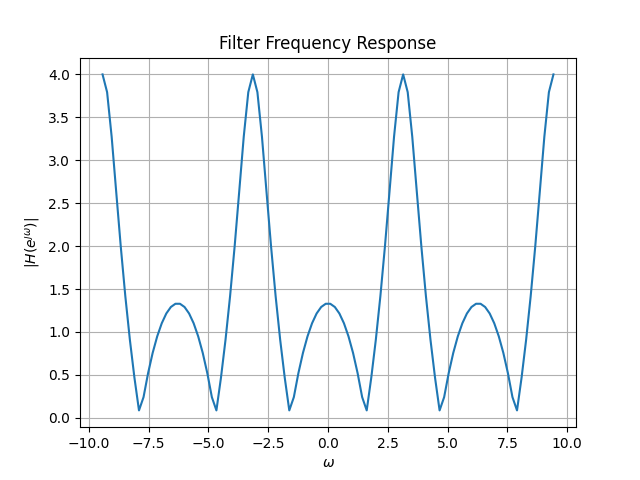
\includegraphics[width=\columnwidth]{/home/naresh/signal processing/figures/dtft.png}
\caption{$\abs{H\brak{e^{\j\omega}}}$}
\label{fig:dtft}
\end{figure}
The period of the numerator is $\pi$ and the denominator is $2\pi$ taking the L.C.M of numerator and the denominator we get
period as $2\pi$

\item Express h(n) in terms of $H(e^{2w})$ .\\
\solution 
 \begin{align}
  &\int_{-\pi}^{\pi} H(e^{\j\omega}) e^{\j\omega n} {d\omega} \\
  &= \int_{-\pi}^{\pi} \sum_{k=-\infty}^\infty h(k)  e^{-\j\omega k} e^{\j\omega n} {d\omega} \\
  &= \sum_{k=-\infty}^\infty h(k) \int_{-\pi}^{\pi} e^{\j\omega(n-k)} {d\omega}
 \end{align}
 
 Now,
 \begin{align}
   \int_{-\pi}^{\pi} e^{\j\omega(n-k)} {d\omega} 
   &= \begin{cases}
    \int_{-\pi}^\pi {d\omega} & n-k = 0 \\
    \left.\frac{\exp\brak{\j\omega(n-k)}}{\j(n-k)}\right|_{-\pi}^\pi & n-k \ne 0
   \end{cases} \\   
   &= \begin{cases}
    2\pi & n-k = 0 \\
    0 & n-k \ne 0
   \end{cases} \\
   &= 2\pi \delta(n-k)
 \end{align}
 
 Thus,
 \begin{align}
  \int_{-\pi}^{\pi} H(e^{\j\omega}) e^{\j\omega n} {\omega} &= 2\pi\sum_{k=-\infty}^\infty h(k) \delta(n-k) \\
  &= 2\pi h(n) * \delta(n) \\
  &= 2\pi h(n)
 \end{align}
 
 Therefore, $h(n)$ is given by the inverse DTFT (IDTFT) of $H\brak{e^{\j\omega}}$
 \begin{align}
  h(n) &= \frac{1}{2\pi} \int_{-\pi}^{\pi} H(e^{\j\omega}) e^{\j\omega n}  {\omega} 
 \end{align}
\end{enumerate}
%

\section{Impulse Response}
\begin{enumerate}[label=\thesection.\arabic*]

\item Using long division, 
find
  \begin{align}
   h(n), \quad n < 5
  \end{align}
  for H(z) in 
  \eqref{eq:freq_resp}.\\
\solution 
 \begin{equation}
  H(z) = \frac{1 + z^{-2}}{1 + \frac12 z^{-1}}
 \end{equation}
 Substitute $z^{-1} = x$
 \polylongdiv{1+x^2}{1+\frac12 x}
 
 \begin{align}
  &\implies 1 + z^{-2} = \brak{1 + \frac12 z^{-1}}\brak{-4 + 2z^{-1}} + 5 \\
  &\implies H(z) = -4 + 2z^{-1} + \frac{5}{1 + \frac12 z^{-1}}
 \end{align}
 
 On applying the inverse $Z$-transform on both sides of the equation
 \begin{align}
  H(z) &\ztrans h(n) \\
  -4 &\ztrans -4\delta(n) \\
  2z^{-1} &\ztrans 2\delta(n - 1) \\
  \frac{5}{1 + \frac12 z^{-1}} &\ztrans 5\brak{-\frac12}^n u(n) \\
 \end{align}
 
 Therefore,
 \begin{equation}
  h(n) = -4\delta(n) + 2\delta(n - 1) + 5\brak{-\frac12}^n u(n)
 \end{equation}

\item Find an expression for $h(n)$ using $H(z)$, given that 
           %in Problem \ref{eq:ztransab} and \eqref{eq:anun}, given that
      \begin{equation}
        \label{eq:impulse_resp}
        h(n) \ztrans H(z)
      \end{equation}
      and there is a one to one relationship between $h(n)$ and $H(z)$. $h(n)$ is known as the {\em impulse response} of the system defined by $\eqref{eq:iir_filter}$.\\ 
    \solution The $H\brak{z}$ can be written as,
      \begin{align}
         H\brak{z} &= \frac{1}{1 + \frac{z^{-1}}{2}} + \frac{z^{-2}}{1+\frac{z^{-1}}{2}}
      \end{align}
      From $\eqref{eq:anun}$ we can write it as,
      \begin{align}
        h\brak{n} &= \brak{\frac{-1}{2}}^{n} u\brak{n} + \brak{\frac{-1}{2}}^{n-2} u\brak{n-2}\label{eq:hn}
      \end{align}
      
    
\item Sketch $h(n)$. Is it bounded? Justify Theoritically.\\
    \solution  Download the code for the plot $\ref{hn}$ from the below link,
     \begin{lstlisting}
wget https://github.com/NareshBandaru13/EE3900-A1/blob/main/codes/5-3.py
     \end{lstlisting}
     \begin{figure}[ht!]
      \centering
      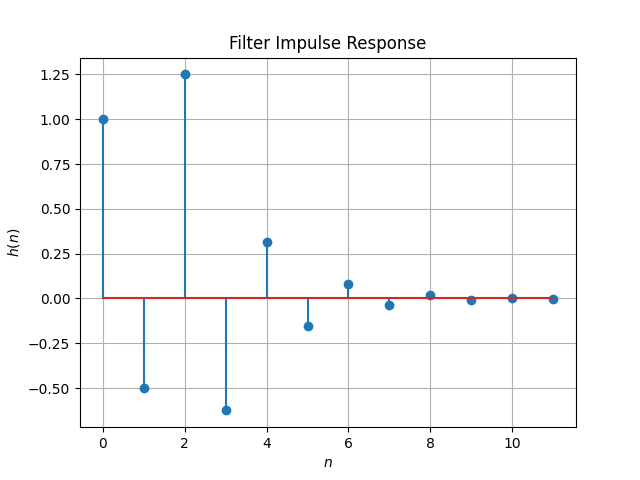
\includegraphics[width = \columnwidth]{/home/naresh/signal processing/figures/hn.png}
      \caption{$h\brak{n}$ as inverse of $H\brak{n}$}     
      \label{hn}
     \end{figure}
     From the plot it seems like $h(n)$ is bounded and becomes smaller in magnitude as $n$ increases.\\
    Using $\eqref{eq:hn}$, we can get theoritical expression as, 
     \begin{align}
       h\brak{n} &= \begin{cases}
                        0 &, n < 0\\
                        \brak{\frac{-1}{2}}^n &, 0\leq n<2\\
                        5\brak{\frac{-1}{2}}^n &, n \geq 2
                     \end{cases}\label{eq:hn_theo}
     \end{align}
    A sequence $\cbrak{x_n}$ is said to be bounded if and only if there exist a positive real number $M$ such that,
         \begin{align}
           \abs{x_n} \leq M , \forall n \in \mathcal{N}\label{def:bounded}
         \end{align}      
    So to say $h\brak{n}$ is bounded we should able to find the $M$ which satisfies $\eqref{def:bounded}$.\\
    For $n < 0$, 
       \begin{align}
    \abs{h\brak{n}} \leq 0 
       \end{align}
    For $0 \leq n <2$,
       \begin{align}
        \abs{h\brak{n}} &= \abs{\frac{-1}{2}}^{n}\\
                        &= \brak{\frac{1}{2}}^{n} \leq 1
       \end{align}
    And for $n \geq 2$,
       \begin{align}
        \abs{h\brak{n}} &= \abs{5\brak{\frac{-1}{2}}}^{n}\\
                        &= \brak{\frac{5}{2}}^{n} \leq \frac{5}{4}
       \end{align}
    From above three cases, we can get $M$ as,
      \begin{align}
        M &= max\cbrak{0,1,\frac{5}{4}} \\
          &= \frac{5}{4}
      \end{align}
    Therefore, $h\brak{n}$ is bounded using $\eqref{def:bounded}$ with $M = \frac{5}{4}$ i.e.,
    \begin{align} 
      \abs{h(n)} \leq \frac{5}{4}  \forall n \in \mathcal{N}
    \end{align}    
    
     
\item Convergent? Justify using the ratio test.\\
     \solution We can say a given real sequence $\cbrak{x_n}$ is convergent if 
       \begin{align}
         \lim_{n \rightarrow \infty}\abs{\frac{x_{n+1}}{x_n}} < 1
       \end{align}
        This is known as Ratio test.\\
      In this case the limit will become,
       \begin{align}
         \lim_{n \rightarrow \infty}\abs{\frac{h\brak{n+1}}{h\brak{n}}} &= \lim_{n \rightarrow \infty}\abs{\frac{5\brak{\frac{-1}{2}}^{n+1}}{5\brak{\frac{-1}{2}}^{n}}} \\
          &= \lim_{n \rightarrow \infty}\abs{\frac{-1}{2}}\\
          &= \frac{1}{2}
       \end{align}
      As $\frac{1}{2} < 1$, from root test we can say that $h\brak{n}$ is convergent.
      
\item The system with $h(n)$ is defined to be stable if
     \begin{equation}
      \sum_{n=-\infty}^{\infty}h(n) < \infty
     \end{equation}
        Is the system defined by $\eqref{eq:iir_filter}$ stable for the impulse response in $\eqref{eq:impulse_resp}$?\\
        
\solution From $\eqref{eq:hn}$,
      \begin{align}
        \sum_{n=-\infty}^{\infty}h\brak{n} &= \sum_{n=-\infty}^{\infty}\brak{\brak{\frac{-1}{2}}^{n} u\brak{n} + \brak{\frac{-1}{2}}^{n-2} u\brak{n-2}}\\
                                           &= 2\brak{\frac{1}{1+\frac{1}{2}}}\\
                                           &= \frac{4}{3}
      \end{align}
       $\therefore$ the system is stable. 
        
\item Verify the above result using a python code.\\
\solution Download the python code from the below link 
    \begin{lstlisting}
  wget https://github.com/NareshBandaru13/EE3900-A1/blob/main/codes/5-6.py
    \end{lstlisting}
  Then run the following command,
    \begin{lstlisting}
  python3 5-6.py
    \end{lstlisting} 
   
   
   
\item Compute and sketch $h(n)$ using 
     \begin{equation}
      \label{eq:iir_filter_h}
      h(n) + \frac{1}{2}h(n-1) = \delta(n) + \delta(n-2), 
     \end{equation}
        This is the definition of $h(n)$.\\
    \solution Download the code for the plot \ref{hndef} from the below link,
     \begin{lstlisting}
wget https://github.com/NareshBandaru13/EE3900-A1/blob/main/codes/5-7.py
     \end{lstlisting}
     Note that this is same as $\ref{hn}$.\\
     \begin{figure}[ht!]
      \centering
      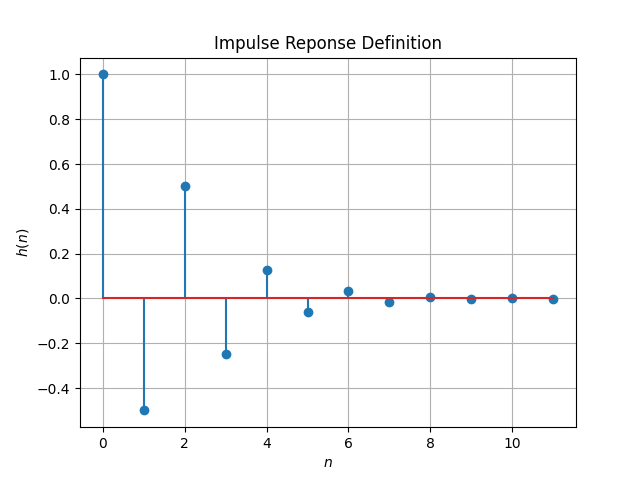
\includegraphics[width = \columnwidth]{/home/naresh/signal processing/figures/hndef.png}
      \caption{From the definition of $h(n)$}
      \label{hndef}
     \end{figure}
    For $n <0$, $h\brak{n} = 0$ and,
     \begin{align} 
       h\brak{0} &= \delta\brak{0}\\
                 &= 1
     \end{align}
    For $n =1$,
     \begin{align} 
       h\brak{1} + \frac{1}{2}h\brak{0} &= \delta\brak{1} + \delta\brak{-1}\\
      \implies  h\brak{1}&= -\frac{1}{2}h\brak{0}\\
                         &= -\frac{1}{2}
     \end{align}
    $n=2$,
      \begin{align}
        h\brak{2} + \frac{1}{2}h\brak{1} &= 0 + \delta\brak{0}\\
              h\brak{2} &= 1 + \frac{1}{4}\\
                        &= \frac{5}{4}
      \end{align}
    And for $n>2$ RHS will be $0$ so,
      \begin{align}
        h\brak{n} &= -\frac{1}{2}h\brak{n-1}
      \end{align}
    Overall 
      \begin{align}
         h\brak{n} &= \begin{cases}
                          0  &, n <0 \\
                          1  &, n = 0 \\
                        -\frac{1}{2} &, n=1 \\
                        \frac{5}{4} &, n =2\\
                        -\frac{1}{2}h\brak{n-1} &, n >2
         \end{cases}
         \end{align}
        \item Compute 
     %
     \begin{equation}
     \label{eq:convolution}
     y(n) = x(n)*h(n) = \sum_{k=-\infty}^{\infty}x(k)h(n-k)
     \end{equation}
     %
     Comment. The operation in $\eqref{eq:convolution}$ is known as
     {\em convolution}.\\
     %
     \solution Download the code for plot $\ref{ynconv}$ from the below link
      \begin{lstlisting}
wget https://github.com/NareshBandaru13/EE3900-A1/blob/main/codes/5-8.py
      \end{lstlisting}
      \begin{figure}[ht!]
        \centering
        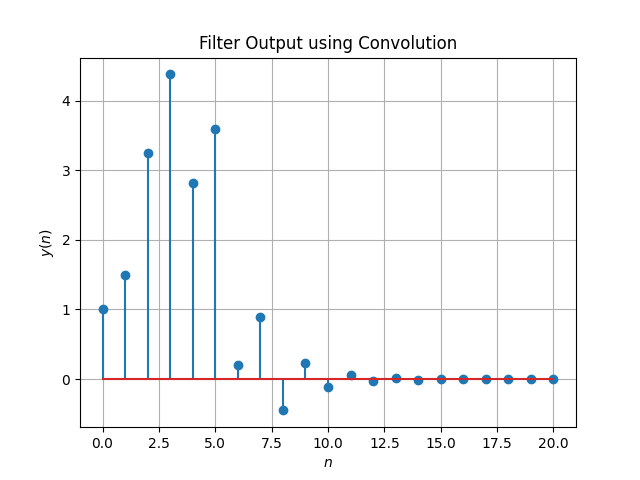
\includegraphics[width = \columnwidth]{/home/naresh/signal processing/figures/ynconv.png}
        \caption{$y(n)$ using the convolution definition}
        \label{ynconv}
      \end{figure}
    \item Express the above convolution using a Toeplitz matrix.\\
    \solution Download the python code from the below link for the plot $\ref{ynconv_toep}$,
     \begin{lstlisting}
wget https://github.com/NareshBandaru13/EE3900-A1/blob/main/codes/5-9.py
     \end{lstlisting}
    Then run the following command,
     \begin{lstlisting}
python3 5-9.py
     \end{lstlisting}
    From $\eqref{eq:convolution}$,we express $y\brak{n}$ as
     \begin{align}
       y\brak{n} &= \sum_{k = -\infty}^{\infty}x\brak{k}h\brak{n-k}
     \end{align}
    To understand how we can use a Toeplitz matrix, we will see what we are doing in $\eqref{eq:convolution}$ 
     \begin{align}
      y\brak{0} &= x\brak{0}h\brak{0}\\
      y\brak{1} &= x\brak{0}h\brak{1} + x\brak{1}h\brak{0}\\
      y\brak{2} &= x\brak{0}h\brak{2} + x\brak{1}h\brak{1} + x\brak{2}h\brak{0}\\
      . \nonumber&\\ 
      .& \nonumber
     \end{align}
    The same thing can be written as,
     \begin{align}
       y\brak{0} &= \myvec{h\brak{0} & 0 & 0 &.\,&.\,&.0}\myvec{x\brak{0}\\x\brak{1}\\x\brak{2}\\ . \\.\\x\brak{5}}\\
       y\brak{1} &= \myvec{h\brak{1} & h\brak{0} & 0 & 0 &.\,&.\,&.0}\myvec{x\brak{0}\\x\brak{1}\\x\brak{2}\\ . \\.\\x\brak{5}}\\
       y\brak{2} &= \myvec{h\brak{2} & h\brak{1} & h\brak{0} & 0& .\,&.0}\myvec{x\brak{0}\\x\brak{1}\\x\brak{2}\\ . \\.\\x\brak{5}}\\
       . & \nonumber \\
       .& \nonumber
     \end{align}
    Using Toeplitz matrix of $h\brak{n}$ we can simplify it as,
     \begin{align}
       y\brak{n} &= \myvec{h\brak{0} & 0 & 0 &.\,&.\,&.\,0 \\
                           h\brak{1} & h\brak{0} & 0 & .\,&.\,&.\,0 \\
                           h\brak{2} & h\brak{1} & h\brak{0} & .\,&.\,&.\,0 \\
                            &&..\\&&..\\ 0 & 0 &  0 &.\,&.\,&.\, h\brak{m-1}}\myvec{x\brak{0}\\x\brak{1}\\x\brak{2}\\ . \\.\\x\brak{5}}\label{eq:ynconv_toep}
     \end{align}
     Now from $\eqref{def:xn}$ we will take n 
      \begin{align}
          x\brak{n} &= \myvec{1\\2\\3\\4\\2\\1}
      \end{align}
      And from $\eqref{eq:hn_theo}$
      \begin{align} 
        h\brak{n} &= \myvec{1 \\ -0.5 \\ 1.25 \\. \\ . }
      \end{align}
     Now using $\eqref{eq:ynconv_toep}$,
      \begin{align}
        y\brak{n} &= x\brak{n}*h\brak{n}\\
                  &= \myvec{1 & 0 & 0 &.\,&.\,&.\,0 \\
                  -0.5 & 1 & 0 & .\,&.\,&.\,0 \\
                  1.25 & -0.5 & 1 & .\,&.\,&.\,0 \\
                   &&..\\&&..\\ 0 & 0 &  0 &.\,&.\,&.\, }\myvec{x\brak{0}\\x\brak{1}\\x\brak{2}\\ . \\.\\x\brak{5}} \\
                  &= \myvec{1\\1.5\\3.25\\.\\.\\.}
      \end{align}
      \begin{figure}
        \centering
        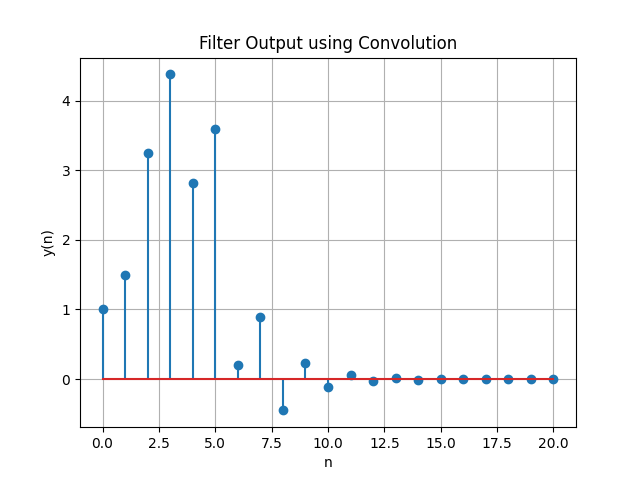
\includegraphics[width = \columnwidth]{/home/naresh/signal processing/figures/ynconv_toeplitz.png}
        \caption{Convolution of $x\brak{n}$ and $h\brak{n}$ using toeplitz matrix}
        \label{ynconv_toep}
       \end{figure}
    \item Show that
     \begin{equation}
      y(n) =  \sum_{k=-\infty}^{\infty}x(n-k)h(k)
      \end{equation}
    \solution Substitute $k := n-k$ in $\eqref{eq:convolution}$, we will get 
     \begin{align}
       y(n) &= \sum_{k=-\infty}^{\infty}x(k)h(n-k)\\
            &= \sum_{n - k=-\infty}^{\infty}x(n-k)h(k)\\
            &= \sum_{k = -\infty}^{\infty}x(n-k)h(k)\\
     \end{align}
\end{enumerate}
\end{document}